\section{Power Spectral Density of Individual Signals}

\begin{multicols}{2}
       \begin{figure}[H]
        \centering
        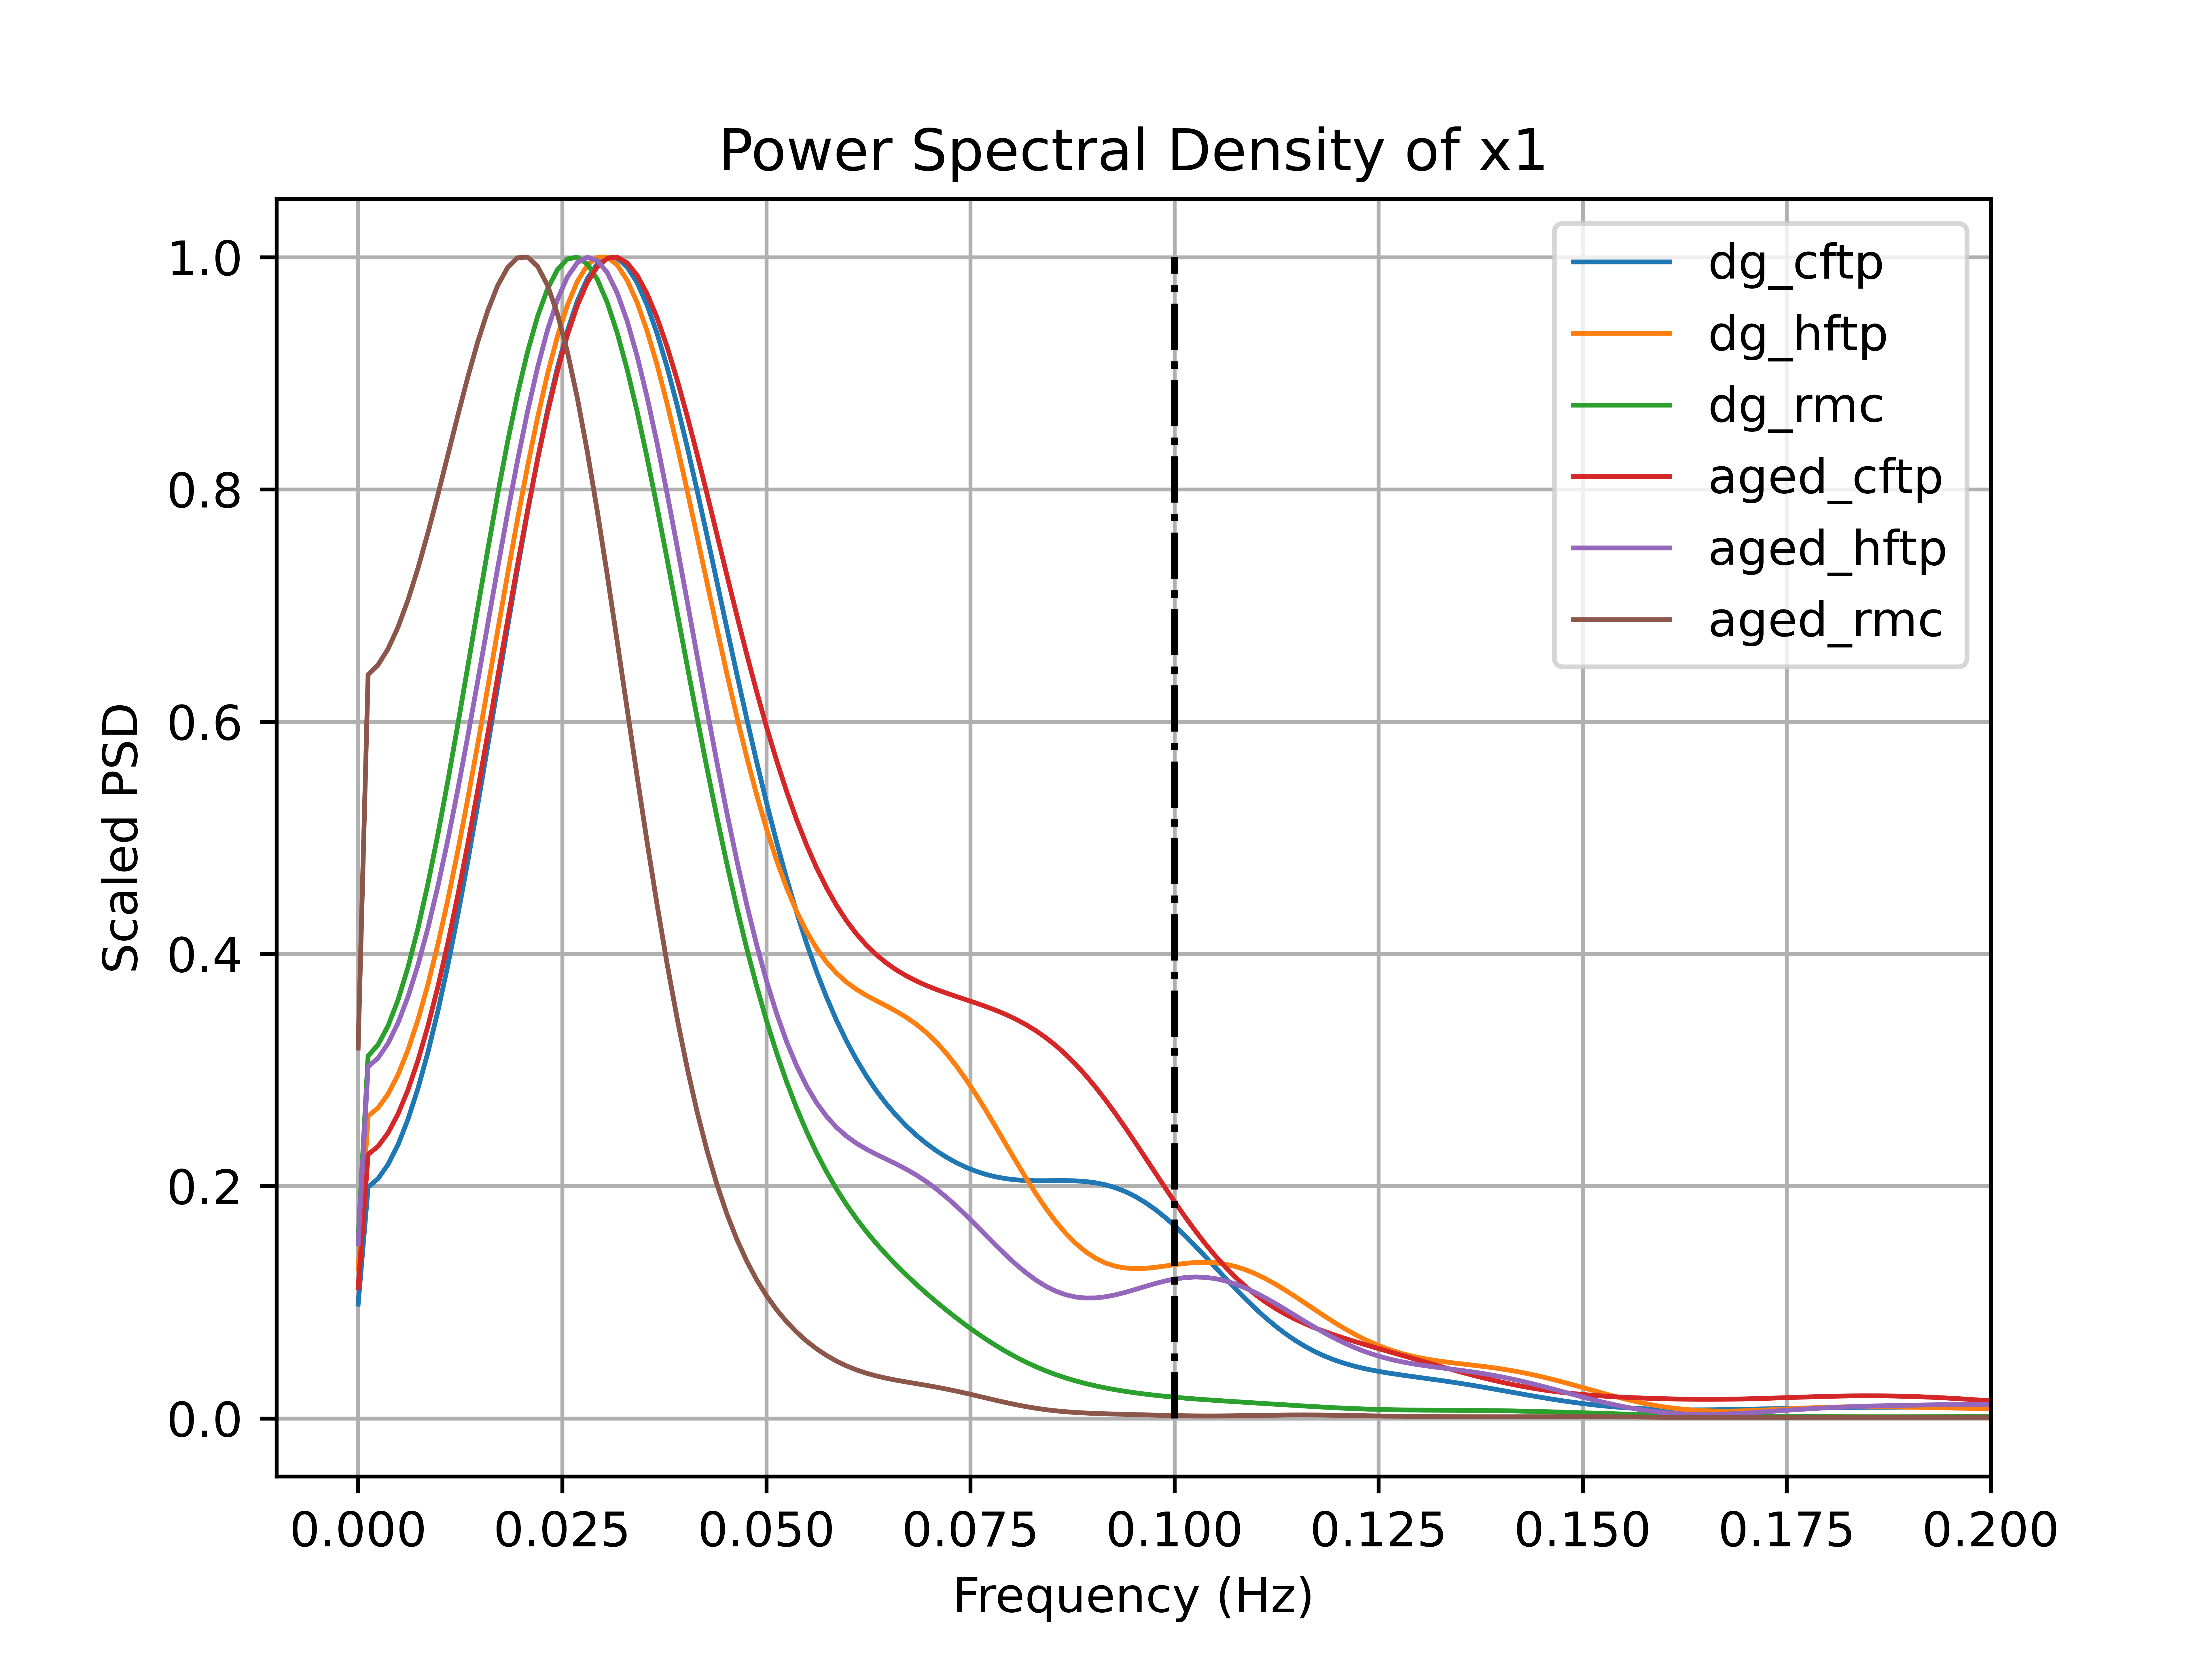
\includegraphics[width=0.48\textwidth]{./figs/bfr_smth/test_psd/x1.png}
        \caption{PSD of $[NO_x]^{out}$ FTIR signal}
       \end{figure}

       \begin{figure}[H]
        \centering
        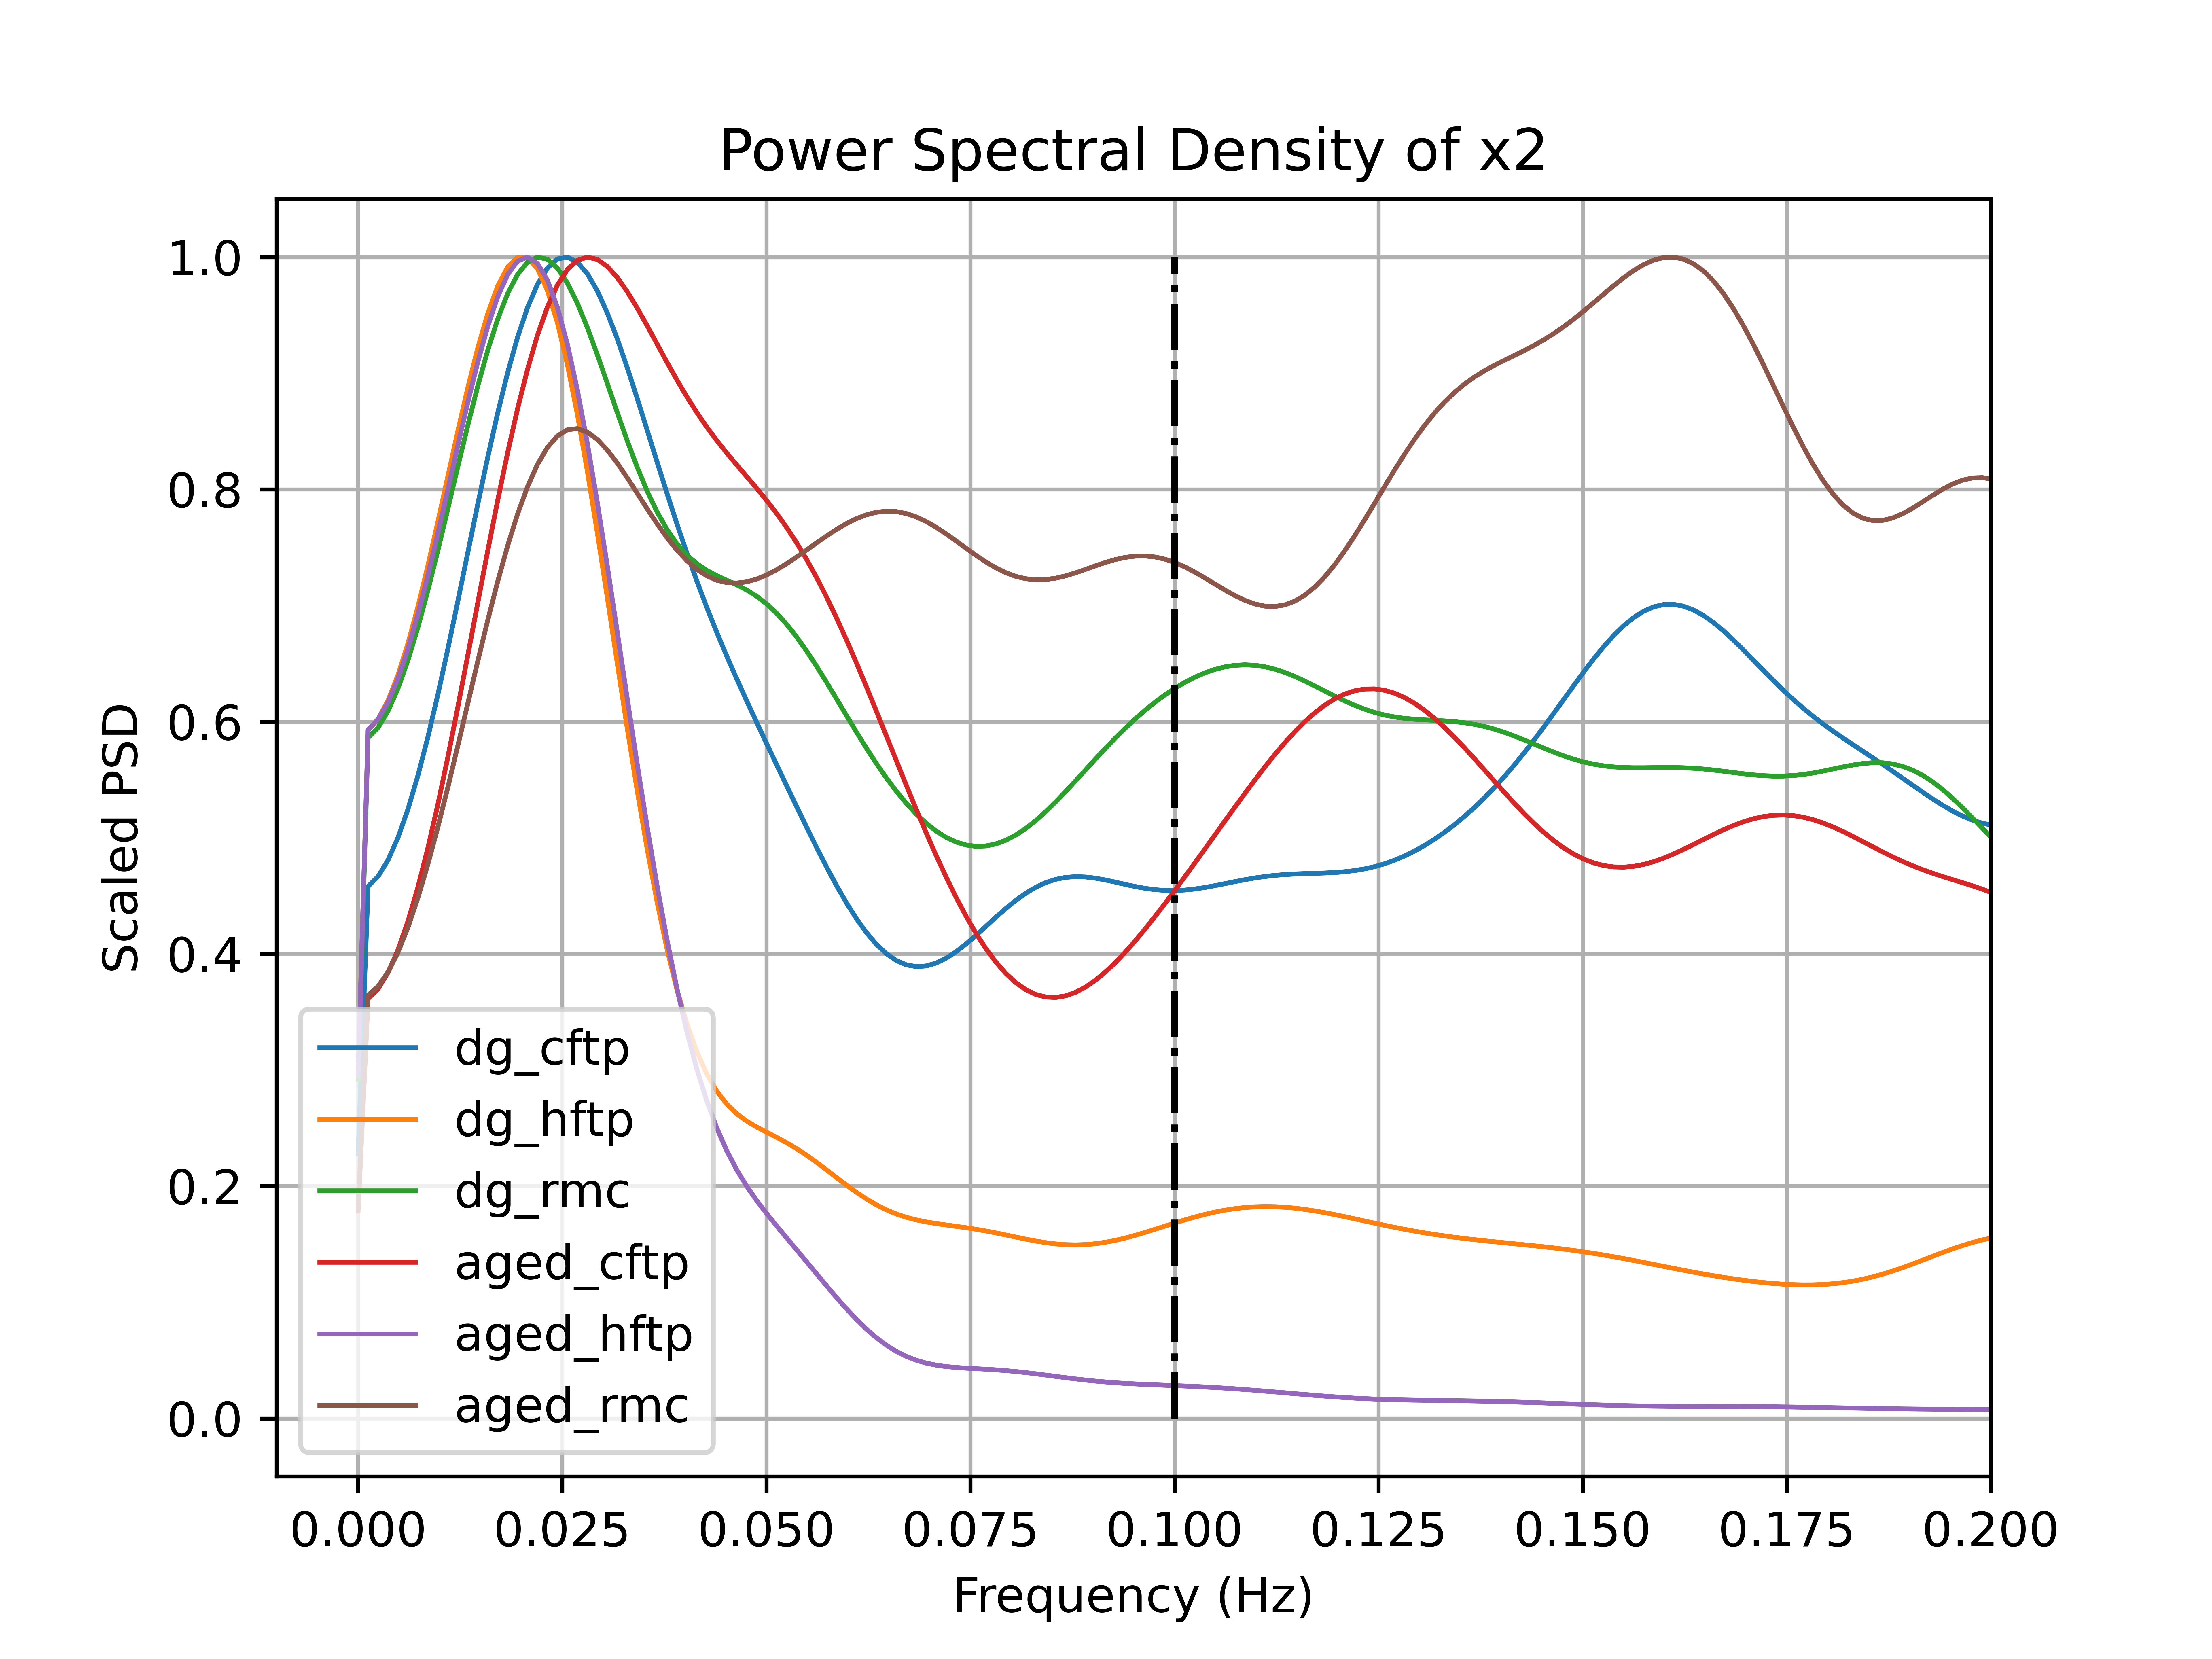
\includegraphics[width=0.48\textwidth]{./figs/bfr_smth/test_psd/x2.png}
        \caption{PSD of $[NH_3]^{out}$ FTIR signal}
       \end{figure}
\end{multicols}
\begin{multicols}{2}
       \begin{figure}[H]
        \centering
        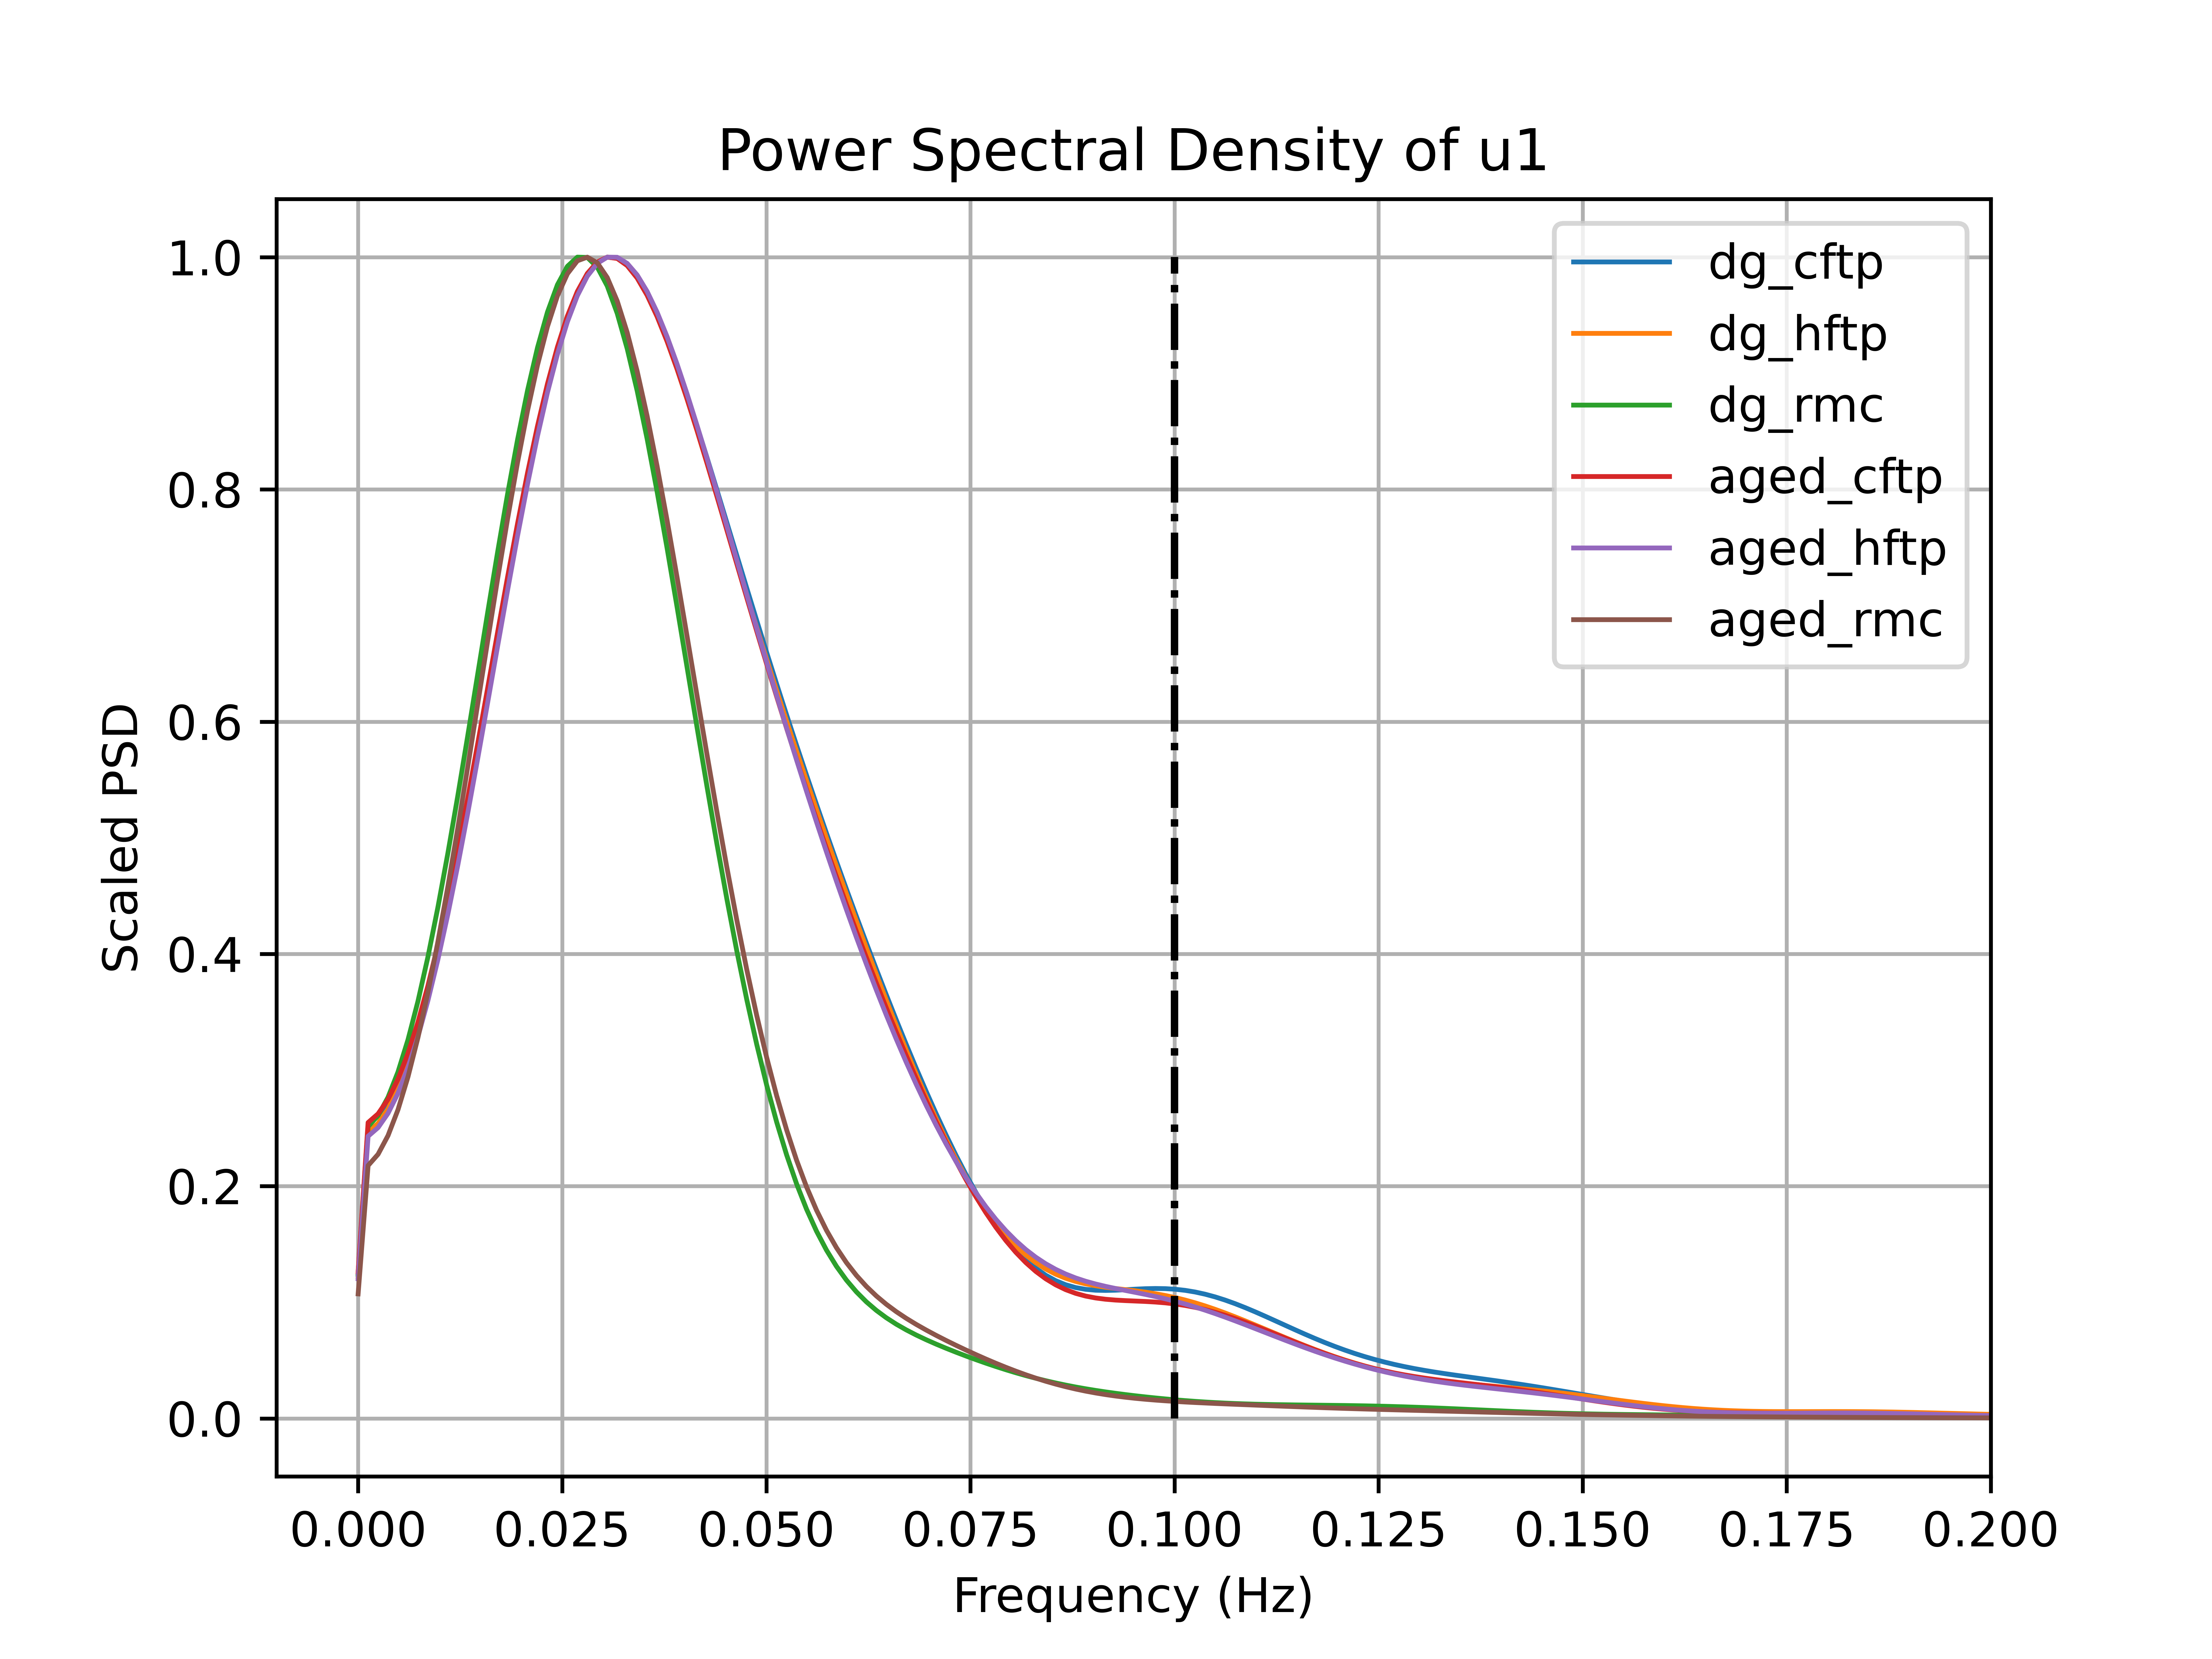
\includegraphics[width=0.48\textwidth]{./figs/bfr_smth/test_psd/u1.png}
        \caption{PSD of $[NO_x]^{in}$ }
       \end{figure}

       \begin{figure}[H]
        \centering
        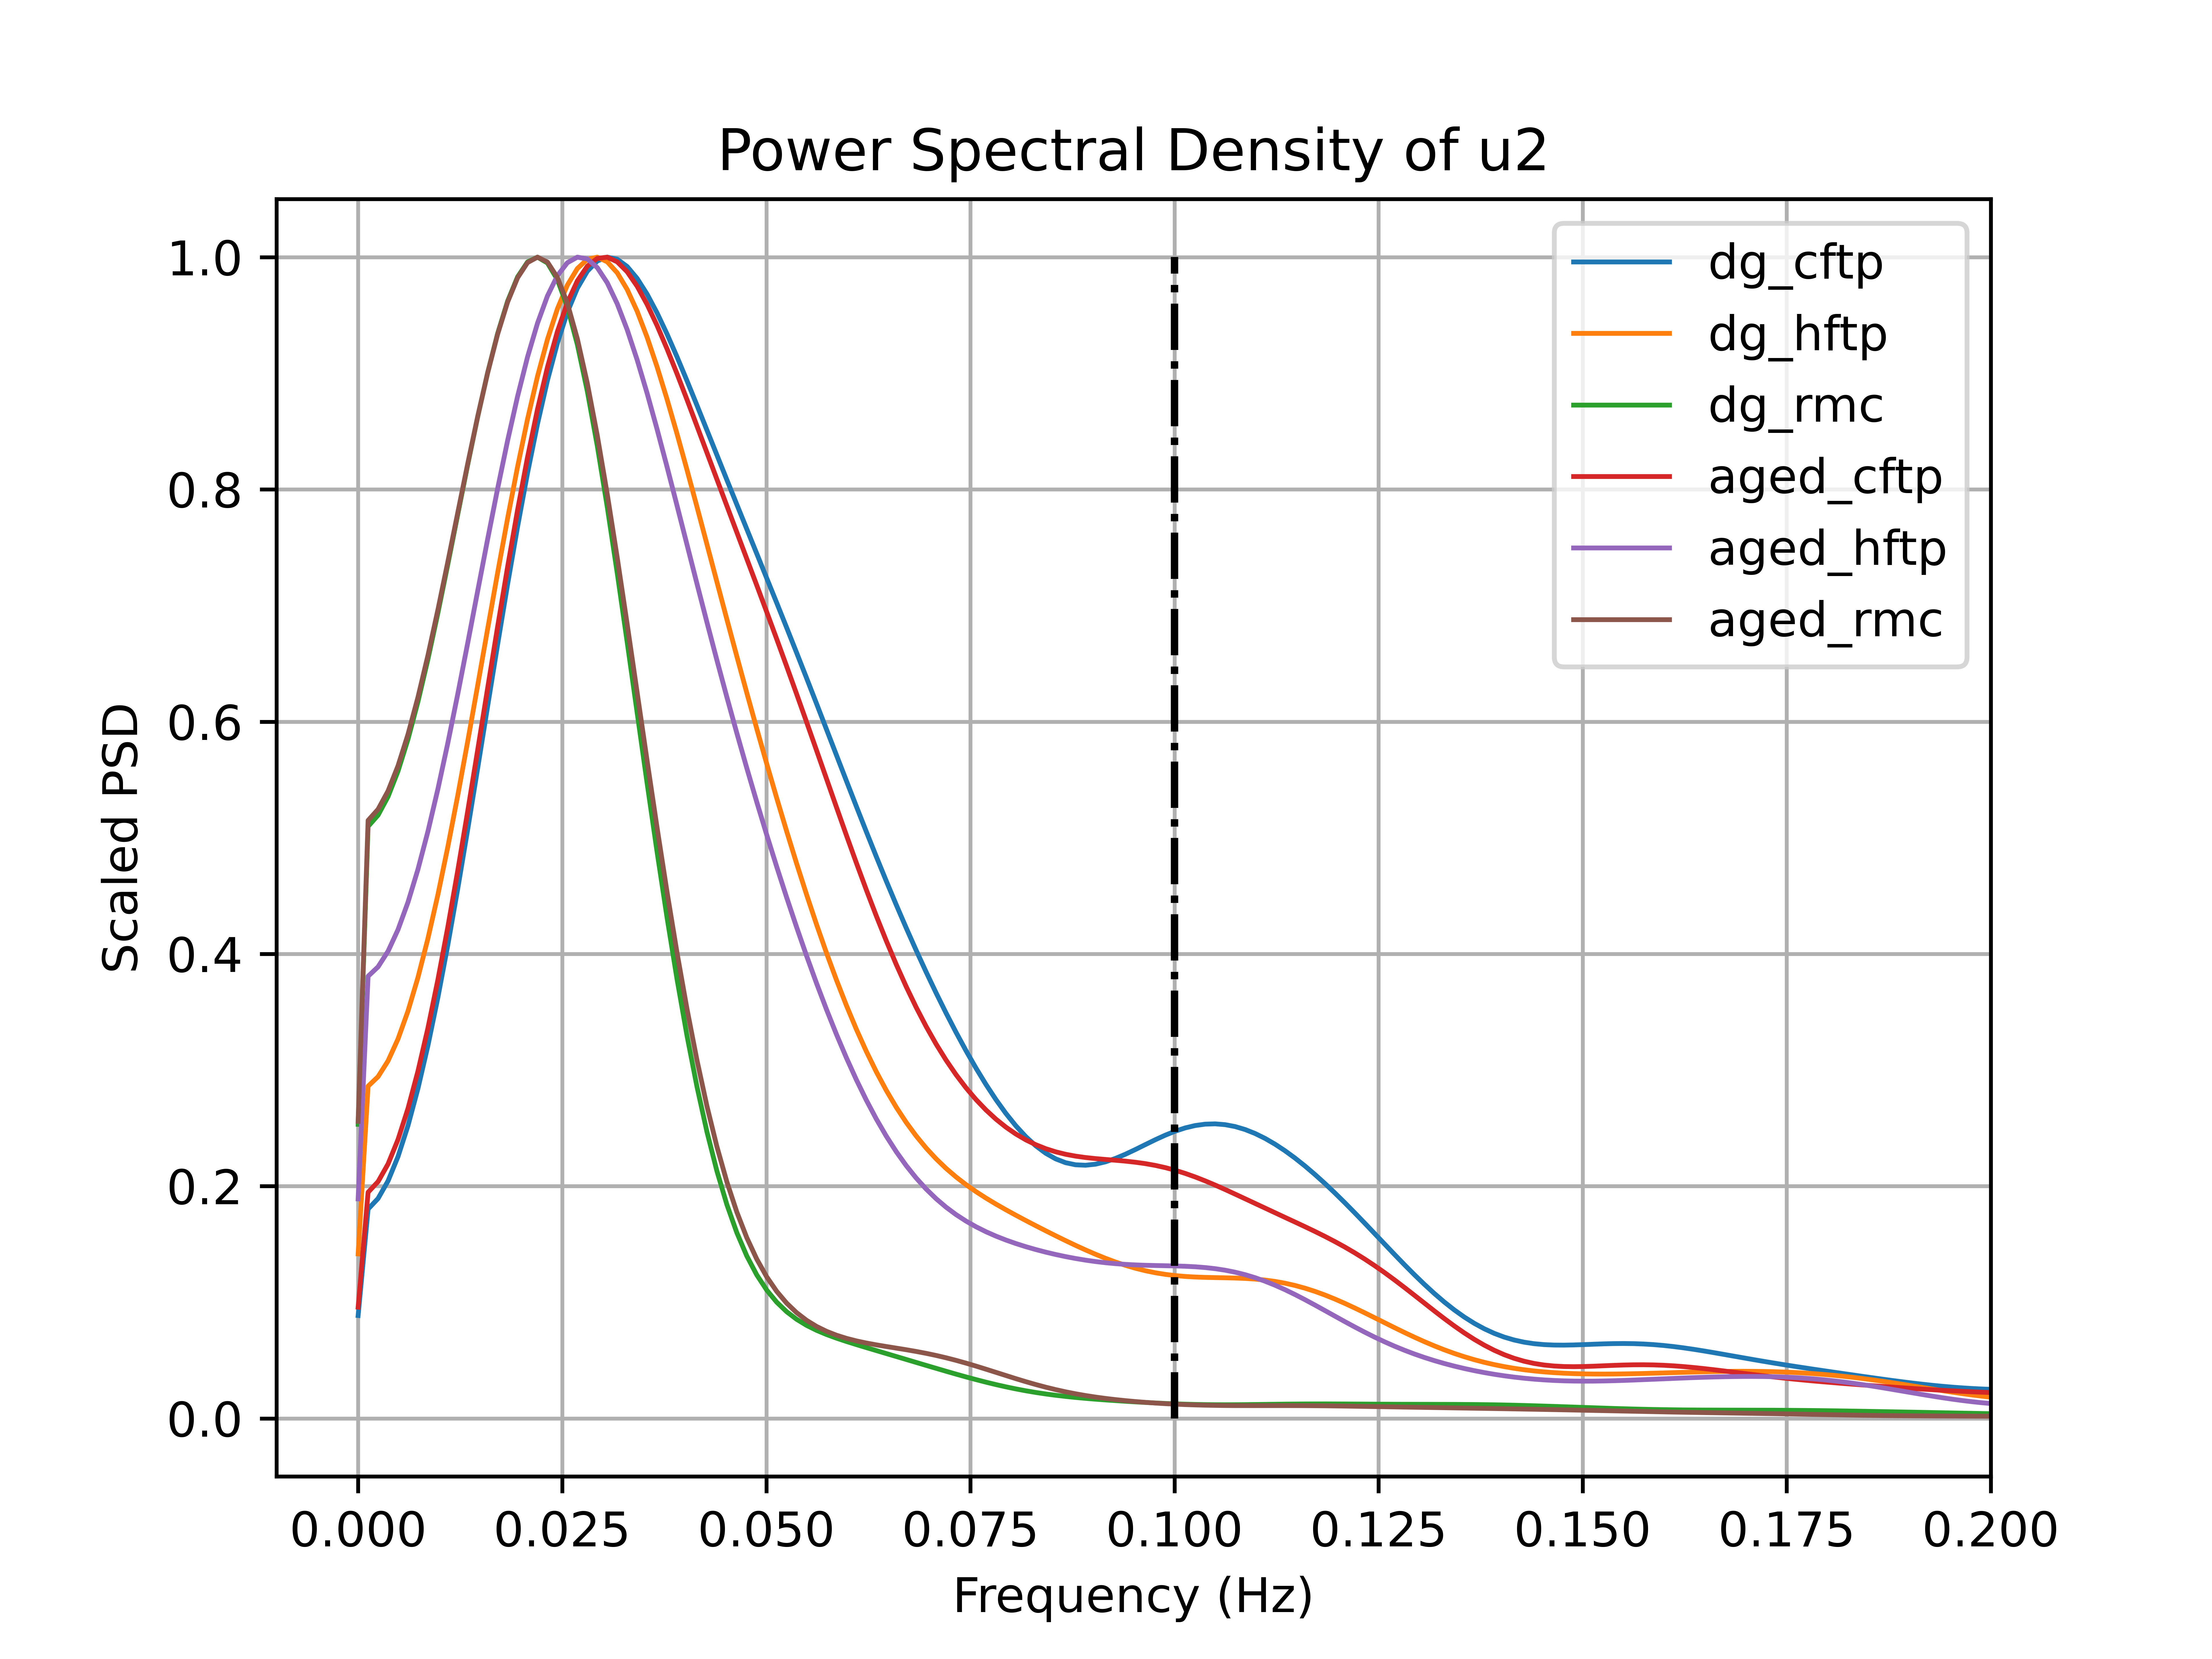
\includegraphics[width=0.48\textwidth]{./figs/bfr_smth/test_psd/u2.png}
        \caption{PSD of urea injection rate}
       \end{figure}
\end{multicols}

\begin{figure}[H]
\centering
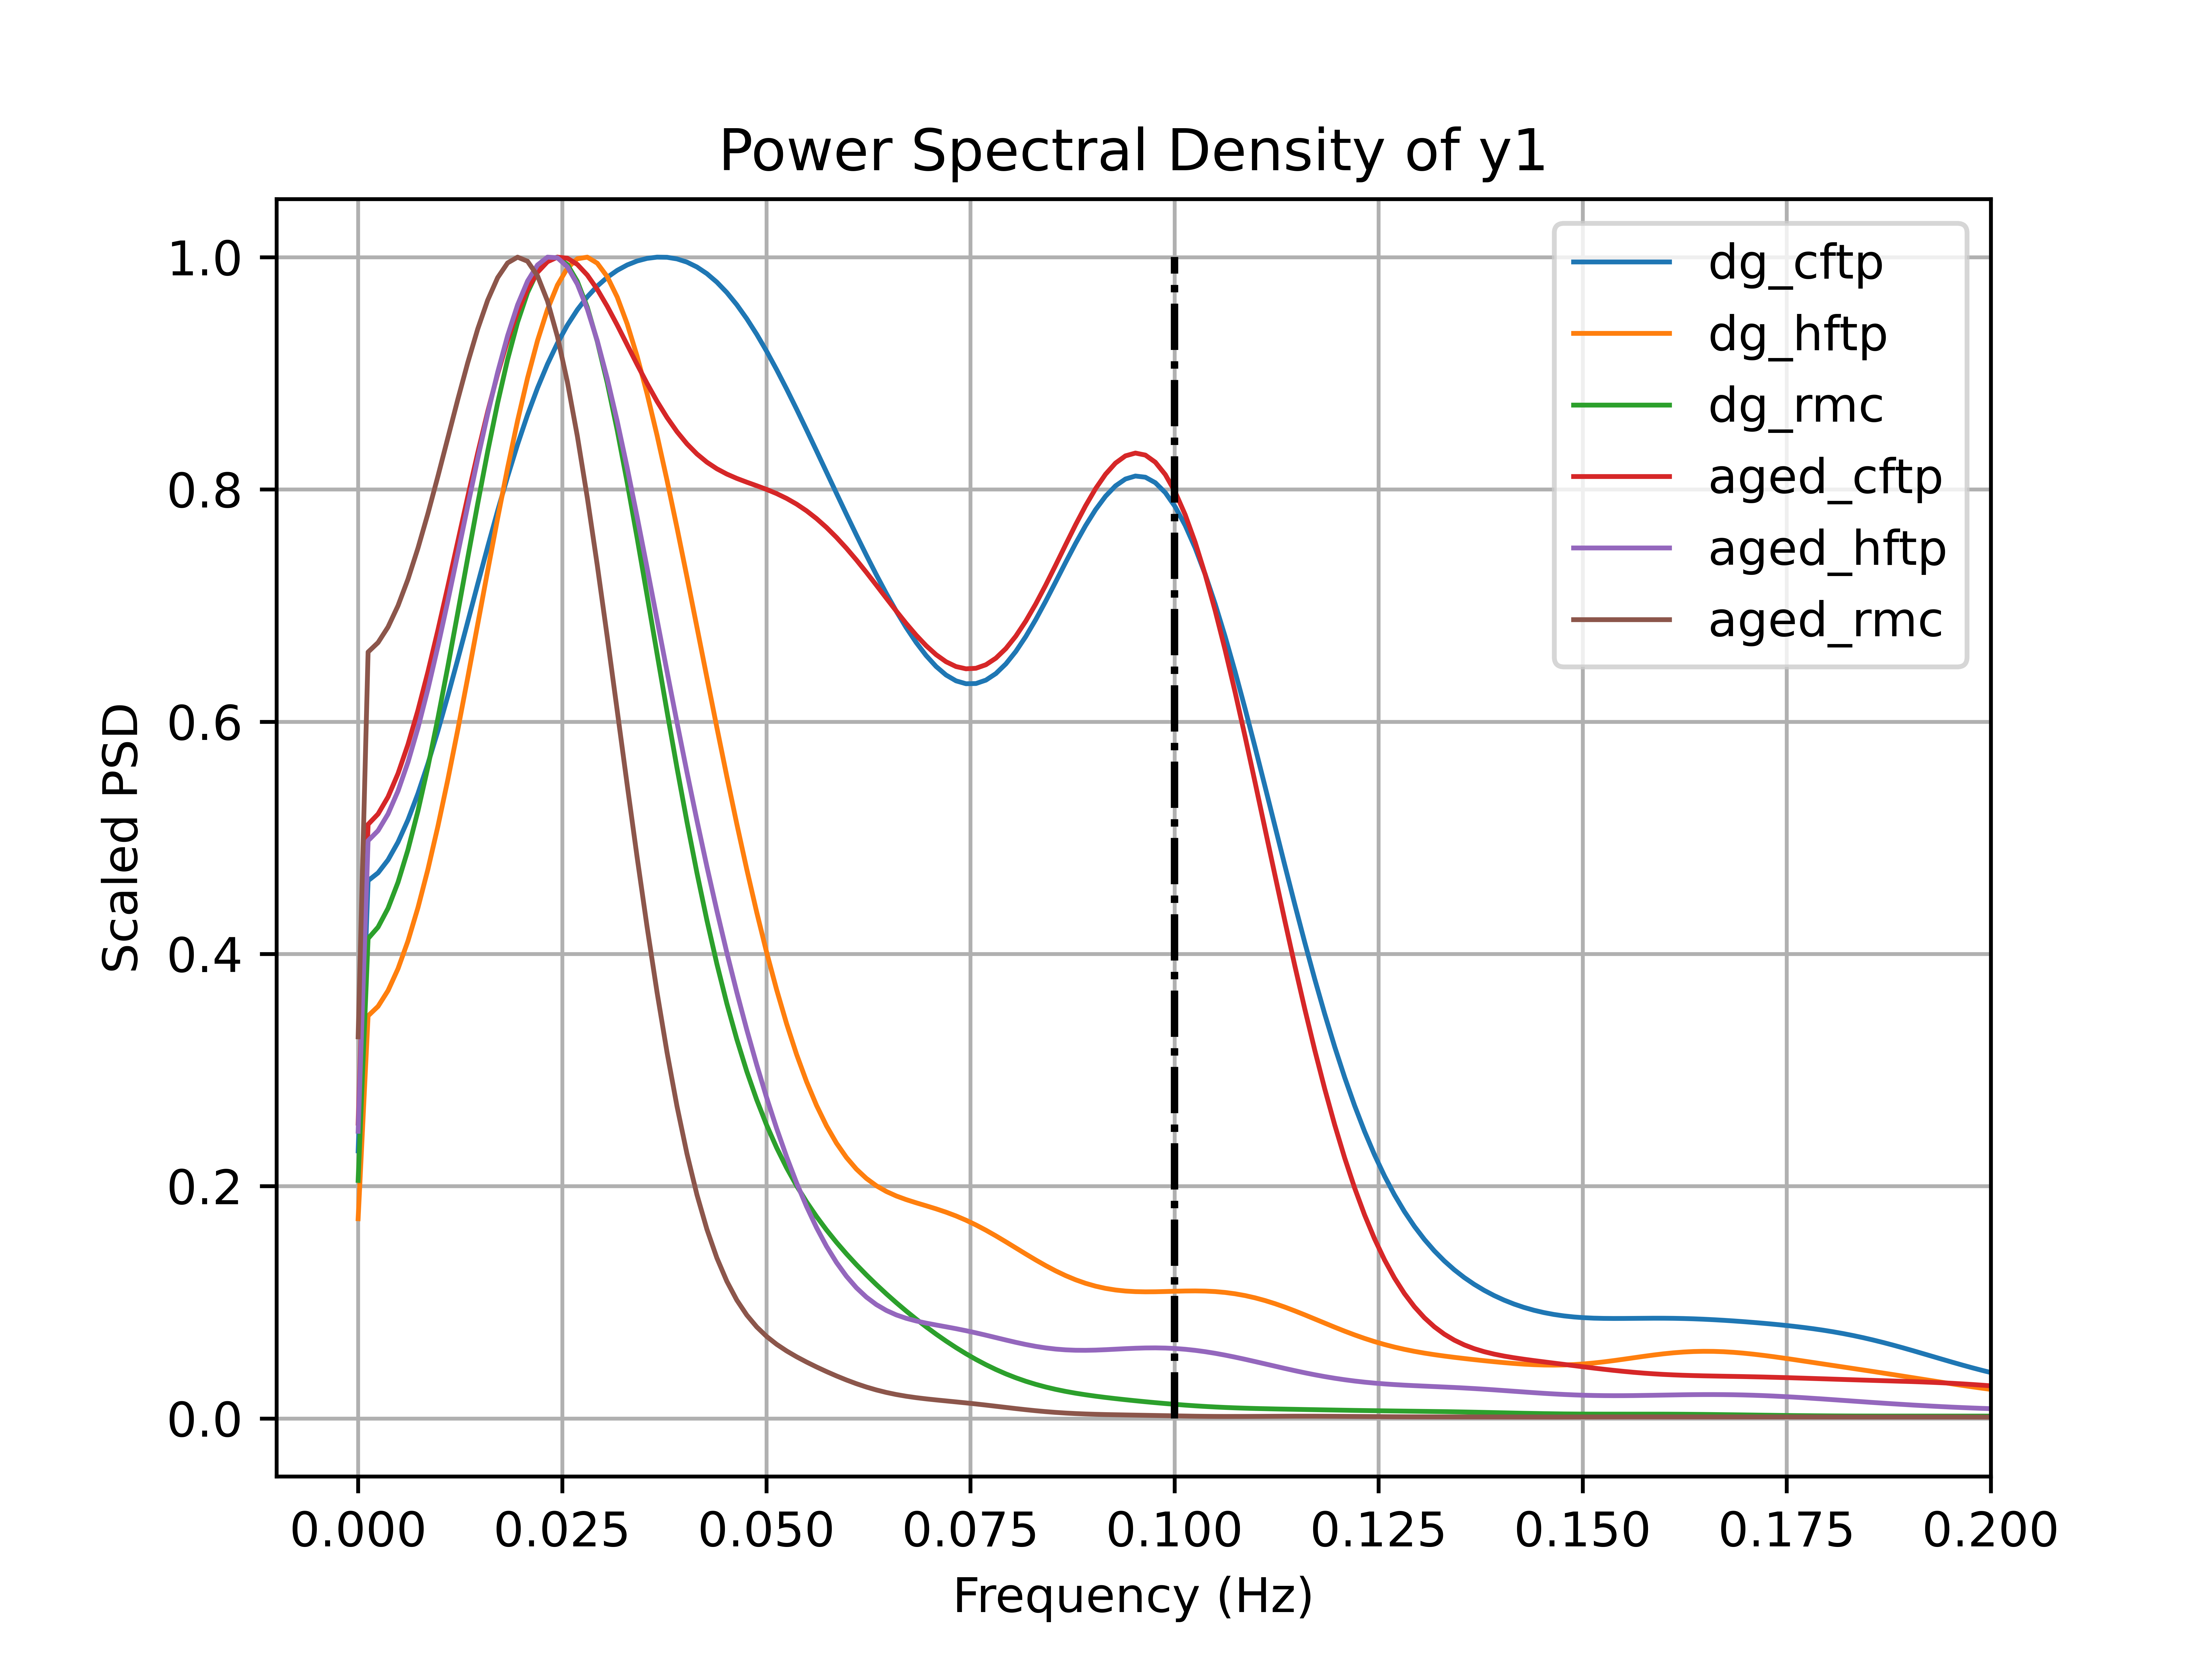
\includegraphics[width=0.6\textwidth]{./figs/bfr_smth/test_psd/y1.png}
\caption{PSD of urea injection rate}
\end{figure}

\begin{multicols}{2}
       \begin{figure}[H]
        \centering
        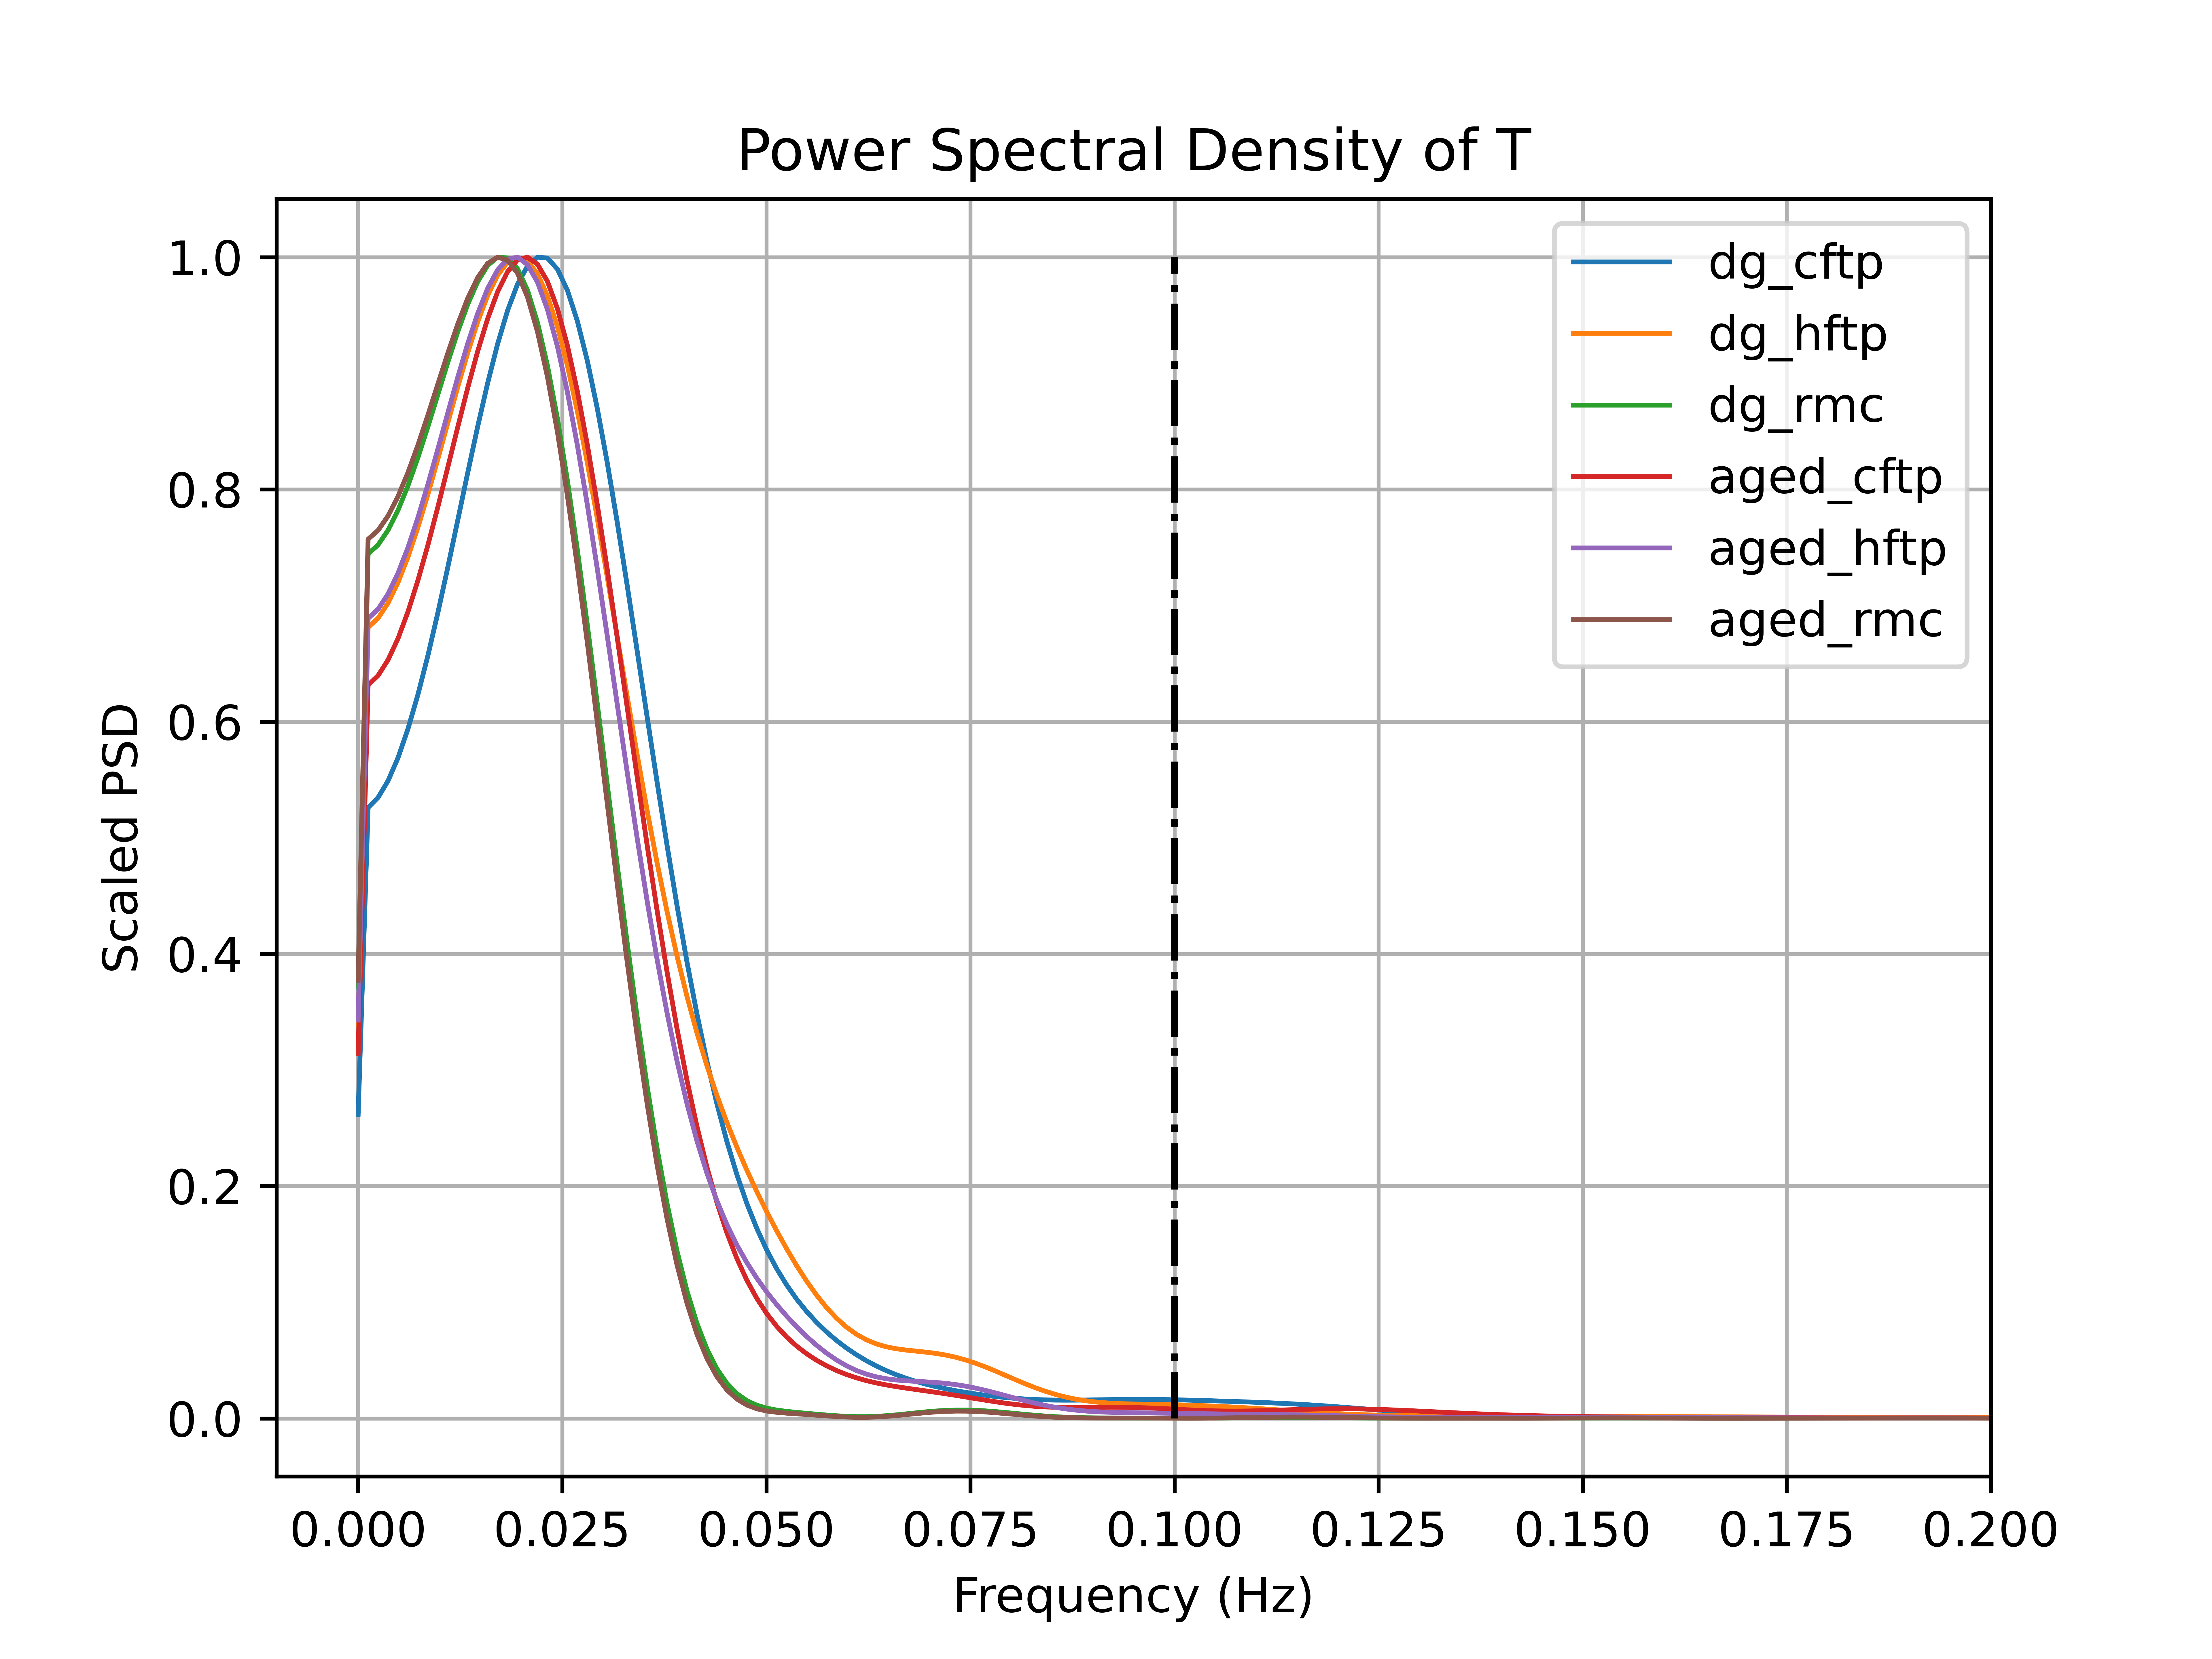
\includegraphics[width=0.48\textwidth]{./figs/bfr_smth/test_psd/T.png}
        \caption{PSD of temperature}
       \end{figure}

       \begin{figure}[H]
        \centering
        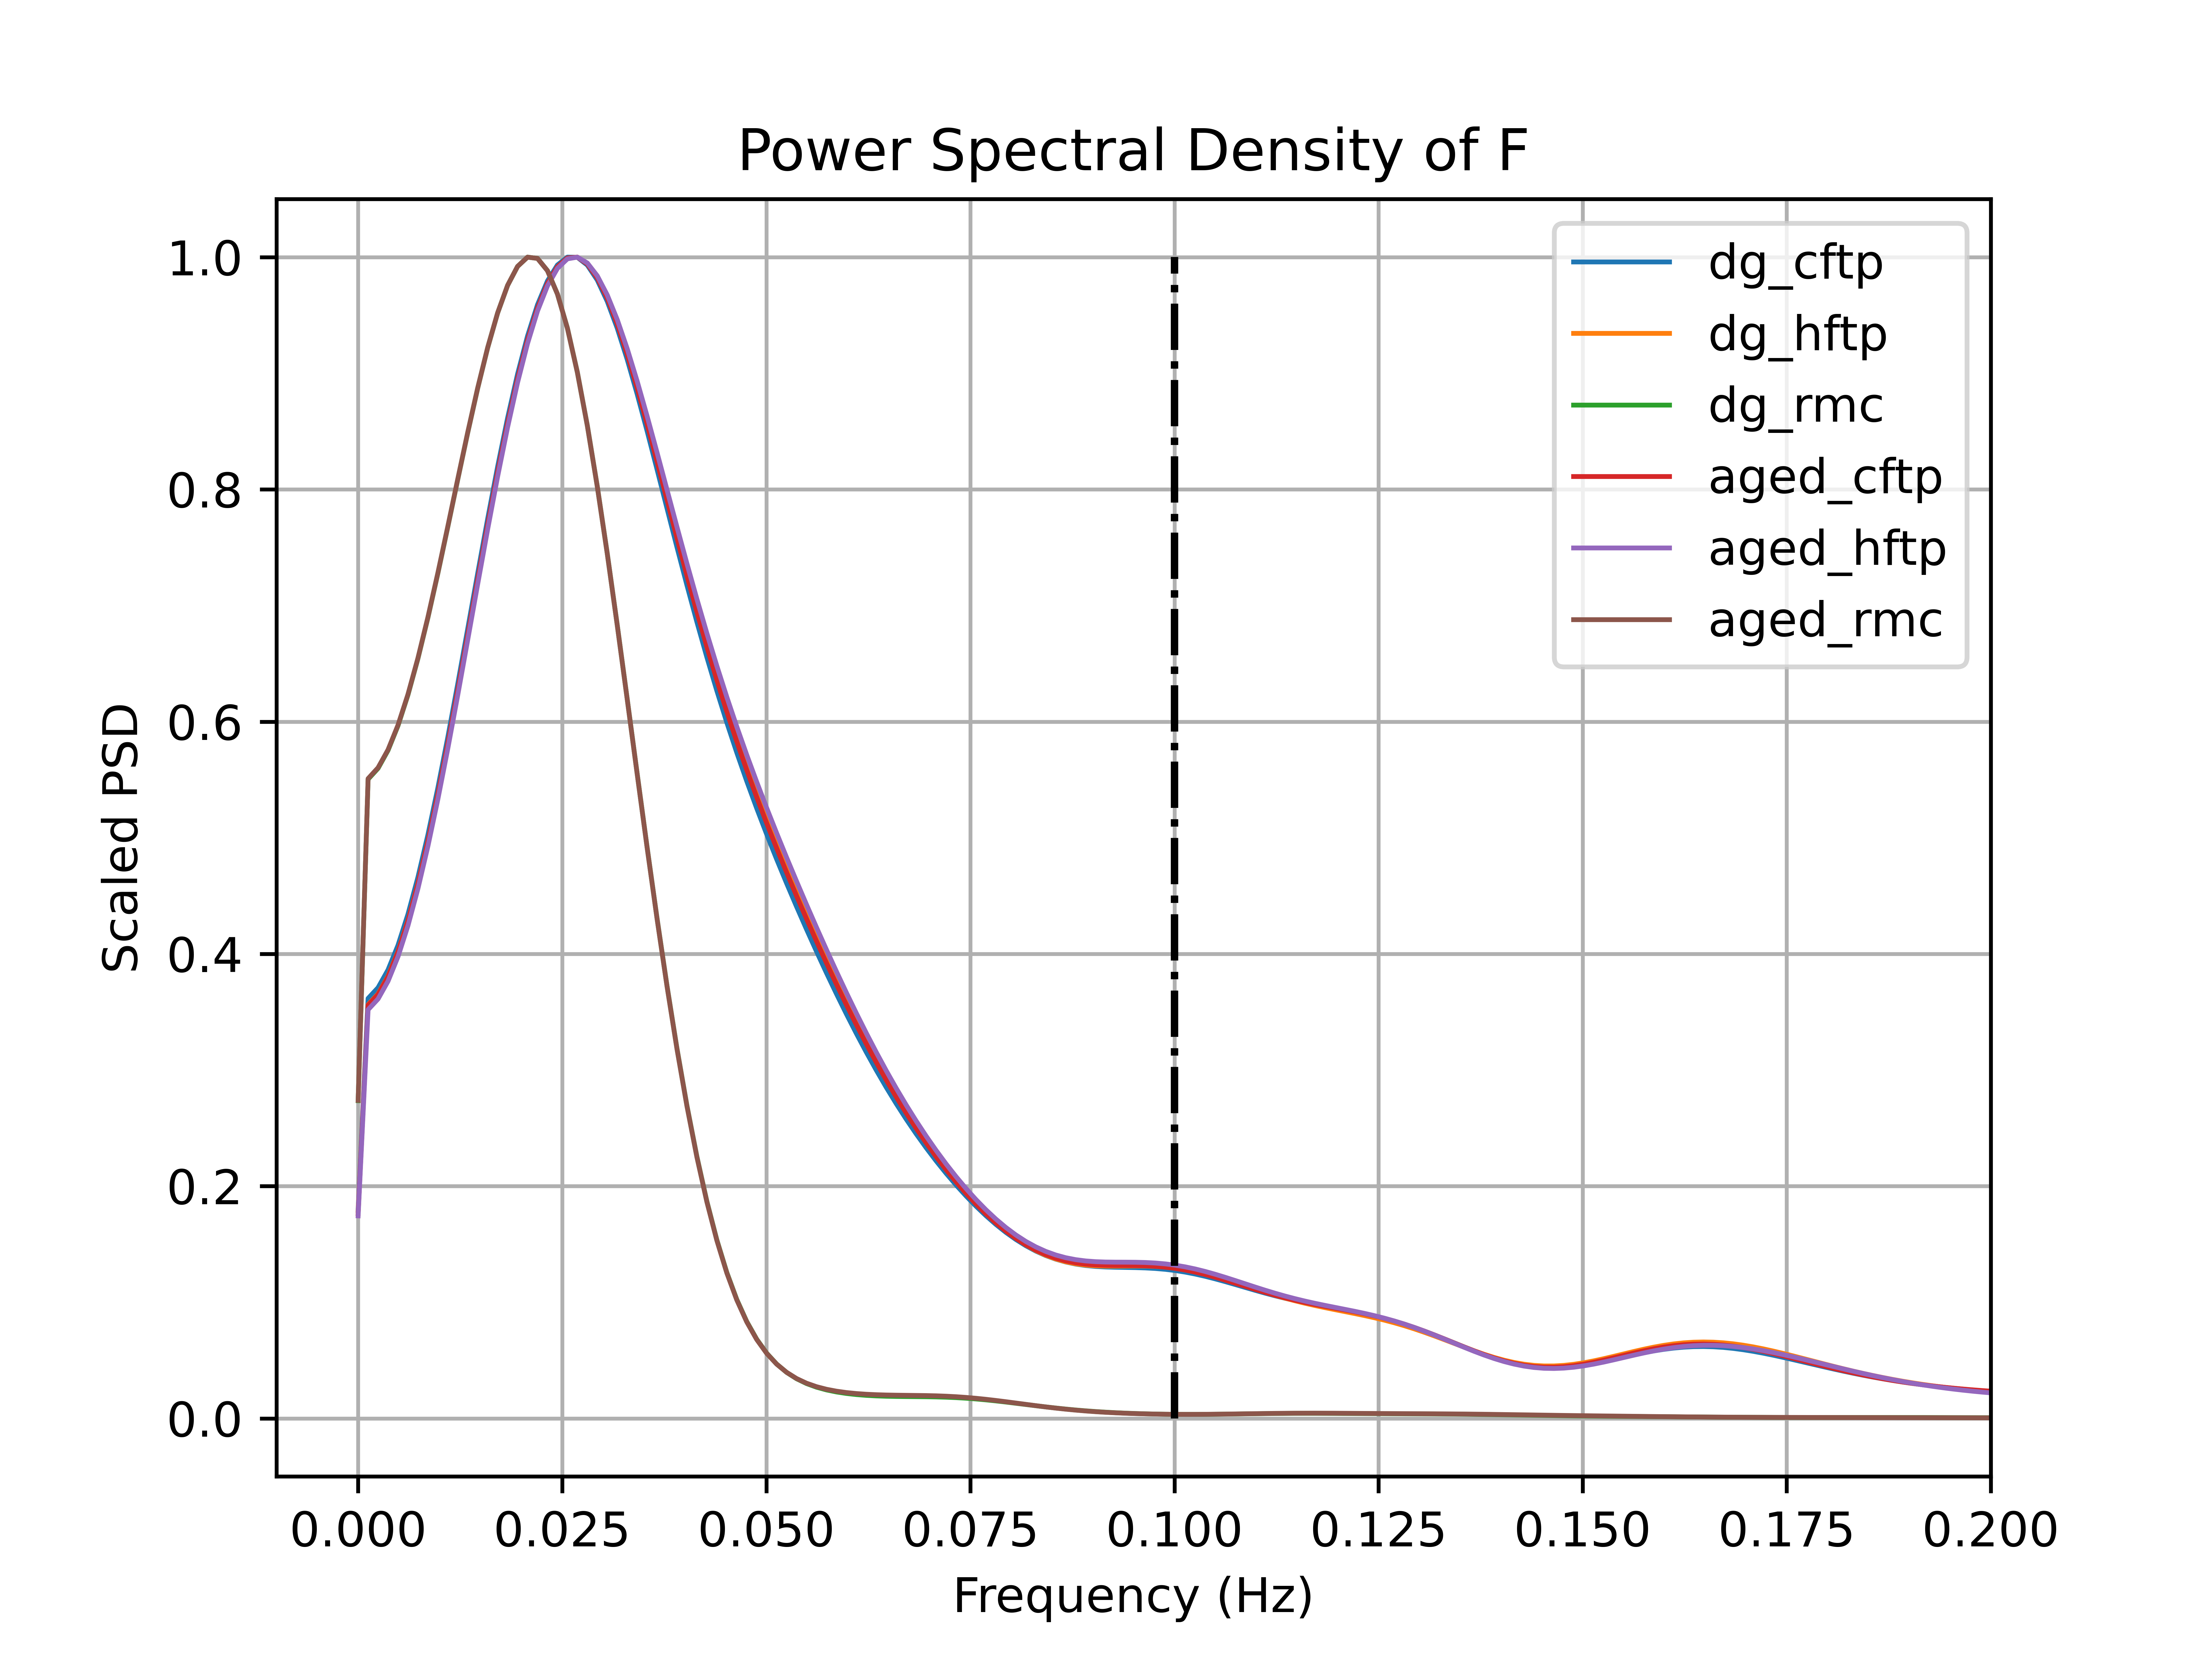
\includegraphics[width=0.48\textwidth]{./figs/bfr_smth/test_psd/F.png}
        \caption{PSD of mass flow rate}
       \end{figure}
\end{multicols}
